\chapter{Manual de usuario}

El manual de usuario se va a realizar para una máquina ubuntu.\\

\section{Instalación de Docker}

En primer lugar instalamos la última versión de docker, \cite{instalacion-docker}. 

Desintalar cualquier versión anterior de Docker.\\

\begin{lstlisting}[language=Bash,caption=Instalación Docker. Parte I, label=cod:suma-cuerpo, style=Consola]
sudo apt-get remove docker docker-engine docker.io containerd runc
\end{lstlisting}


Actualizar los paquetes \texttt{apt} para tener acceso a las últimas actualizaciones e instalar los paquetes que permiten al sistema operativo acceder a los repositorios de Docker a través de HTTPS.\\

\begin{lstlisting}[language=Bash,caption=Instalación Docker. Parte II, label=cod:suma-cuerpo, style=Consola]
$ sudo apt-get update
$ sudo apt-get install apt-transport-https ca-certificates curl gnupg-agent software-properties-common
\end{lstlisting}

Añadir la clave GPG oficial de Docker, la clave GPG es una característica de seguridad para asegurar que el software que se va instalar es auténtico.\\
 
\begin{lstlisting}[language=Bash,caption=Instalación Docker. Parte III, label=cod:suma-cuerpo, style=Consola]
$ curl -fsSL https://download.docker.com/linux/ubuntu/gpg | sudo apt-key add -

OK
\end{lstlisting}

Verificar que obtenemos la clave con la siguiente huella, para ello buscamos la huella con los últimos 8 dígitos, de la misma.\\

\texttt{9DC8 5822 9FC7 DD38 854A  E2D8 8D81 803C 0EBF CD88}\\

\begin{lstlisting}[language=Bash,caption=Instalación Docker. Parte IV, label=cod:suma-cuerpo, style=Consola]
$ sudo apt-key fingerprint 0EBFCD88

pub   rsa4096 2017-02-22 [SCEA]
      9DC8 5822 9FC7 DD38 854A  E2D8 8D81 803C 0EBF CD88
uid           [ unknown] Docker Release (CE deb) <docker@docker.com>
sub   rsa4096 2017-02-22 [S]
\end{lstlisting}

Instalar el repositorio de Docker.\\ 

\begin{lstlisting}[language=Bash,caption=Instalación Docker. Parte V, label=cod:suma-cuerpo, style=Consola]
$ sudo add-apt-repository "deb [arch=amd64] https://download.docker.com/linux/ubuntu $(lsb_release -cs) stable"
\end{lstlisting}

Actualizar los repositorios que se acaban de agregar e instalar la última versión de Docker Engine y Docker Containerd.\\


\begin{lstlisting}[language=Bash,caption=Instalación Docker. Parte VI, label=cod:suma-cuerpo, style=Consola]
$ sudo apt-get update
$ sudo apt-get install docker-ce docker-ce-cli containerd.io
\end{lstlisting}

Verificar que se ha instalado correctamente comprobando la versión de Docker.\\

\begin{lstlisting}[language=Bash,caption=Instalación Docker. Parte VII, label=cod:suma-cuerpo, style=Consola]
$ docker --version

Docker version 19.03.13, build 4484c46d9d
\end{lstlisting}

Algunos comandos útiles para el trabajo con Docker se muestran en el código \ref{cod:cm-docker}.

\begin{lstlisting}[language=Bash,caption=Comandos útiles de Docker, label=cod:cm-docker]
#Muestra los contenedores
$ sudo docker ps

#Lista los contenedores con los IDs
$ sudo docker container ls --all

#Lista las imagenes con los IDs
$ sudo docker images ls --all 

#Guarda los cambios del docker
$ sudo docker commit <ID-CONTAINER> <NOMBRE-NUEVO:ETIQUETA>

#Corre un contenedor, abriendo los puertos indicados
$ sudo docker run -it -p <PUERTO:PUERTO> <NOMBRE:ETIQUETA>

#Elimina un contenedor
$ sudo docker rm <ID-CONTAINER>
\end{lstlisting}

\section{Instalación Blockchain ARK}

En Docker, iniciamos una imagen de ubuntu xenial. Además abrimos los puertos que van a ser necesarios posteriormente 4103, para la API, y 4200, para el explorer.\\

\begin{lstlisting}[language=Bash,caption=Instalación Blockchain. Parte I, label=cod:suma-cuerpo, style=Consola]
$ sudo docker run -ti -p 4103:4103 -p 4200:4200 ubuntu:xenial
\end{lstlisting}

Una vez estamos dentro de la máquina Docker instalamos sudo, para poder trabajar en modo administrador desde el usuario que vamos a crear.\\

\begin{lstlisting}[language=Bash,caption=Instalación Blockchain. Parte II, label=cod:suma-cuerpo, style=Consola]
$ apt-get install sudo
$ adduser deployer

Añadiendo el usuario `deployer' ...
Añadiendo el nuevo grupo `deployer' (1001) ...
Añadiendo el nuevo usuario `deployer' (1001) con grupo `deployer' ...
Creando el directorio personal `/home/deployer' ...
Copiando los ficheros desde `/etc/skel' ...
Introduzca la nueva contraseña de UNIX: ********
Vuelva a escribir la nueva contraseña de UNIX: ********
passwd: contraseña actualizada correctamente
Cambiando la información de usuario para deployer
Introduzca el nuevo valor, o presione INTRO para el predeterminado
	Nombre completo []: 
	Número de habitación []: 
	Teléfono del trabajo []: 
	Teléfono de casa []: 
	Otro []: 
¿Es correcta la información? [S/n] S
\end{lstlisting}

Cambiar el modo del usuario deployer incluyéndolo en el grupo sudo para que sea un superusuario y finalmente, entrar al usuario deployer.\\

\begin{lstlisting}[language=Bash,caption=Instalación Blockchain. Parte III, label=cod:suma-cuerpo, style=Consola]
$ usermod -aG sudo deployer
$ su - deployer
\end{lstlisting}

Actualizamos los paquete e instalamos algunos nuevos como \texttt{git}, \texttt{curl} y \texttt{yarn}.\\

\begin{lstlisting}[language=Bash,caption=Instalación Blockchain. Parte IV, label=cod:suma-cuerpo, style=Consola]
$ sudo apt-get update
$ sudo apt-get install git curl yarn jq apt-transport-https
\end{lstlisting}

Instalar las dependencias nvm.\\

\begin{lstlisting}[language=Bash,caption=Instalación Blockchain. Parte V, label=cod:suma-cuerpo, style=Consola]
$ curl -o- https://raw.githubusercontent.com/creationix/nvm/v0.33.8/install.sh | bash
\end{lstlisting}

Para comprobar que se ha instalado correctamente nos salimos del usuario deployer y volvemos a entrar.\\

\begin{lstlisting}[language=Bash,caption=Instalación Blockchain. Parte VI, label=cod:suma-cuerpo, style=Consola]
$ command -v nvm

nvm
\end{lstlisting}

Para eliminar nvm
\begin{lstlisting}[language=Bash,caption=Instalación Blockchain. Parte VII, label=cod:suma-cuerpo, style=Consola]
$ nvm use system
$ npm uninstall -g a_module
$ sudo npm  install -g npm
\end{lstlisting}

Instalar pm2.\\

\begin{lstlisting}[language=Bash,caption=Instalación Blockchain. Parte VIII, label=cod:suma-cuerpo, style=Consola]
$ sudo apt-get install npm
$ sudo npm i -g pm2
$ ln -s /usr/bin/nodejs /usr/bin/node
\end{lstlisting}

Comando interesantes para trabajar con pm2. Nos servirar para observar si la blockchain y el explorer están levantados.

\begin{lstlisting}[language=Bash,caption=Comandos pm2, label=cod:suma-cuerpo, style=Consola]
#Lista los demonios de pm2
$ pm2 list

#Se obtienen los estados de los demonios de pm2
$ pm2 status
\end{lstlisting}

Clonamos el directorio deployer de \texttt{@ArkEcosystem}.\\

\begin{lstlisting}[language=Bash,caption=Instalación Blockchain. Parte IX, label=cod:suma-cuerpo, style=Consola]
git clone https://github.com/ArkEcosystem/deployer.git
\end{lstlisting}

Iniciar la base de datos e instalar tanto la blockchain como el explorer. Una vez que instalemos el \texttt{core} obtendremos en la salida la dirección y la passphrase del wallet Genesis la tenemos que guardar en un archivo para más tarde poder hacer las transacciones, aún así podemos encontrar la passphrase en el archivo ..... . Esto puede tardar unos minutos
\begin{lstlisting}[language=Bash,caption=Instalación Blockchain. Parte X, label=cod:suma-cuerpo, style=Consola]
$ sudo service postgresql start
$ sudo apt-get update -y 
$ sudo apt-get install -y libjemalloc-dev
$ ./deployer/bridgechain.sh install-core --config deployer/config.sample.conf --autoinstall-deps --non-interactive
\end{lstlisting}

\begin{figure}[h]
	\centering
	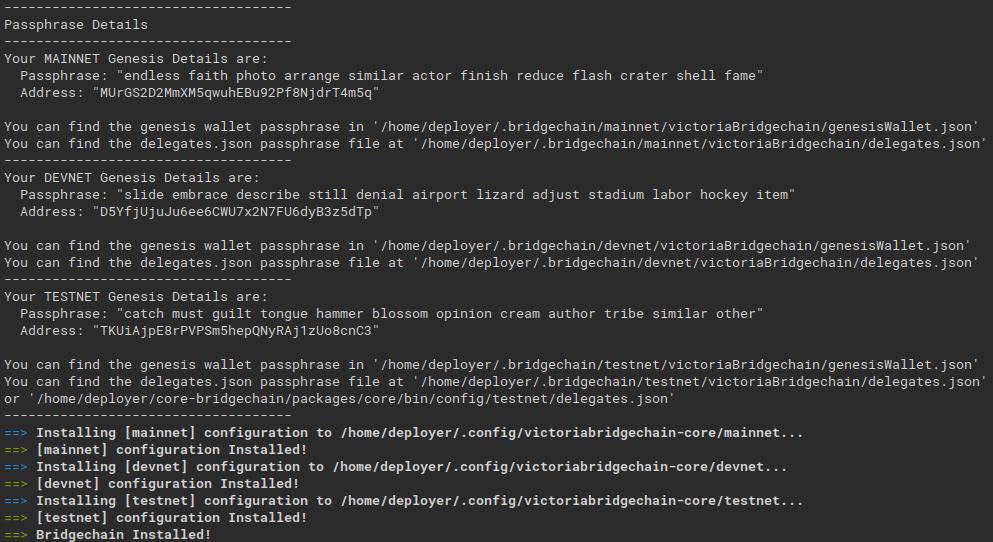
\includegraphics[width=15cm,height=9cm]{figuras/Instalacion_bridgechain.png}
	\caption{Salida tras la instalación del core}
	\label{fig:gantt-real-1}
\end{figure}

\begin{lstlisting}[language=Bash,caption=Instalación Blockchain. Parte X, label=cod:suma-cuerpo, style=Consola]
$ ./deployer/bridgechain.sh install-explorer --config deployer/config.sample.conf --skip-deps --non-interactive
\end{lstlisting}



Iniciamos la blockchain y el explorer.\\

\begin{lstlisting}[language=Bash,caption=Instalación Blockchain. Parte XII, label=cod:suma-cuerpo, style=Consola]
$ ./deployer/bridgechain.sh start-core --network testnet

==> Starting...
Starting victoriabridgechain-relay... done
Starting victoriabridgechain-forger... done
==> Start OK!


$ ./deployer/bridgechain.sh start-explorer --network testnet
\end{lstlisting}

\begin{figure}[h]
	\centering
	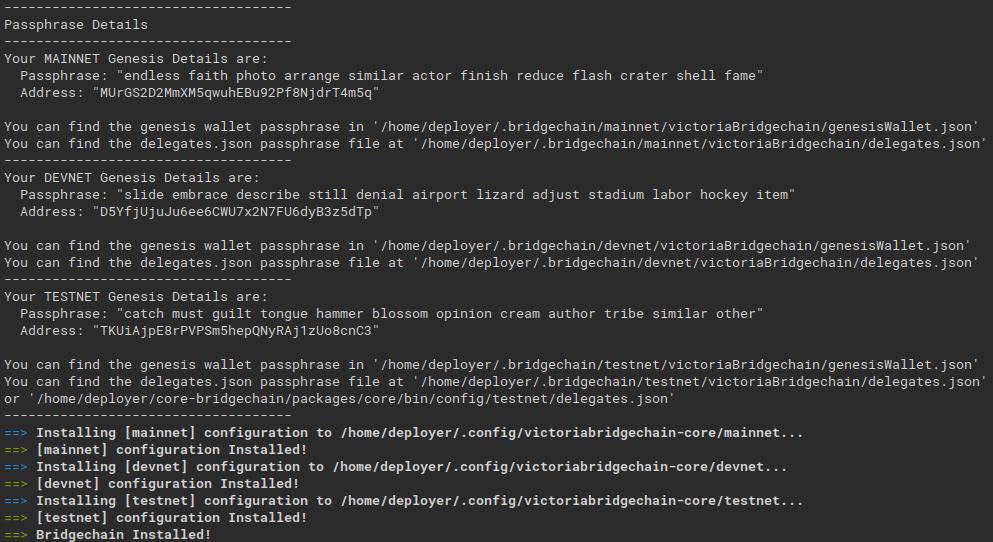
\includegraphics[width=15cm,height=9cm]{figuras/Instalacion_bridgechain.png}
	\caption{Salida tras la instalación del core}
	\label{fig:gantt-real-1}
\end{figure}

\section{Instalación Wallet ARK}





\begin{lstlisting}[language=Bash,caption=Instalación Blockchain. Parte III, label=cod:suma-cuerpo, style=Consola]

\end{lstlisting}


\begin{lstlisting}[language=Bash,caption=Instalación Blockchain. Parte III, label=cod:suma-cuerpo, style=Consola]

\end{lstlisting}

\begin{lstlisting}[language=Bash,caption=Instalación Blockchain. Parte III, label=cod:suma-cuerpo, style=Consola]

\end{lstlisting}

\begin{lstlisting}[language=Bash,caption=Instalación Blockchain. Parte III, label=cod:suma-cuerpo, style=Consola]

\end{lstlisting}

\begin{lstlisting}[language=Bash,caption=Instalación Blockchain. Parte III, label=cod:suma-cuerpo, style=Consola]

\end{lstlisting}

\begin{lstlisting}[language=Bash,caption=Instalación Blockchain. Parte III, label=cod:suma-cuerpo, style=Consola]

\end{lstlisting}









